\documentclass[smaller,compress]{beamer}
\usepackage{amsmath,amsfonts}
\usetheme{Madrid}
\usecolortheme{seagull}
\setbeamertemplate{navigation symbols}{}
\begin{document}
\title{GMM, Indirect Inference and Bootstrap}
\subtitle{Bootstrap}
\author[Willi Mutschler]{Willi Mutschler}
\date{Winter 2015/2016}
\institute{TU Dortmund}
\maketitle

\section{Bootstrap}


\begin{frame}\frametitle{Bootstrap}\small
\begin{block}{Meaning}\scriptsize
verb tr.: To help oneself with one's own initiative and no outside help.\\
noun: Unaided efforts.\\
adjective: Reliant on one's own efforts.\\
\scriptsize (http://wordsmith.org/words/bootstrap.html)
\end{block}
\begin{block}{Etymology}\scriptsize
While pulling on bootstraps may help with putting on one's boots, it's impossible to lift oneself up like that. Nonetheless the fanciful idea is a great visual and it gave birth to the idiom "to pull oneself up by one's (own) bootstraps", meaning to better oneself with one's own efforts, with little outside help. It probably originated from the tall tales of Baron M\"unchausen who claimed to have lifted himself (and his horse) up from the swamp by pulling on his own hair.\\
\scriptsize (http://wordsmith.org/words/bootstrap.html)
\end{block}
\begin{center}
    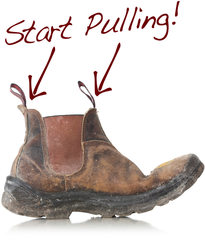
\includegraphics[width=.2\textwidth]{pics/boots.png}
    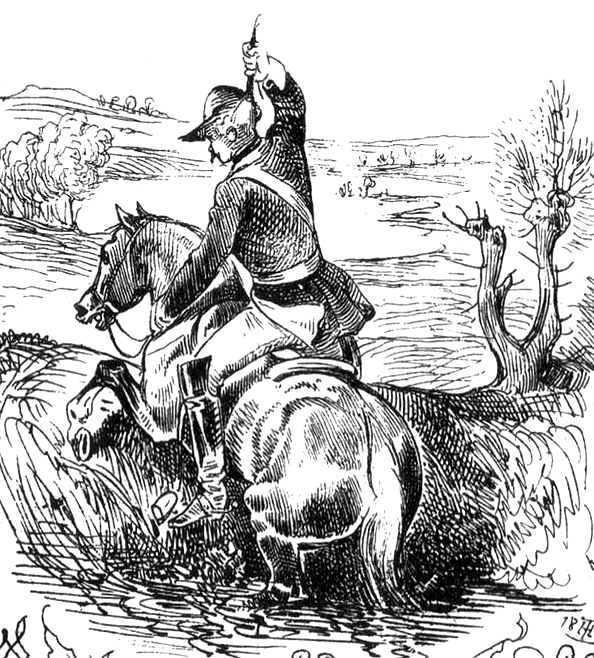
\includegraphics[width=.2\textwidth]{pics/munchhausen.jpg}
\end{center}
\end{frame}


\begin{frame}\frametitle{Bootstrap}\framesubtitle{Basic idea}
\begin{block}{Point of departure}
    \begin{itemize}
      \item Unknown distribution function $F$
      \item Simple random sample $x_{1},\ldots ,x_{n}$ from $F$
      \item Make inference about a population characteristic $\theta$, using a statistic $T$, whose value is $t$ in the sample
      \begin{itemize}
        \item What are bias, standard error or quantiles of $T$?
        \item What are likely values under a certain null hypothesis?
        \item How do we compute confidence intervals?
      \end{itemize}
    \end{itemize}
\end{block}
\begin{block}{Key idea}
  \begin{itemize}
    \item Resample from original data either directly or via a fitted model
    \item Assess variability of quantities of interest from replicate datasets without (long-winded and error-prone) analytical calculation
  \end{itemize}
\end{block}
\end{frame}



\begin{frame}\frametitle{Bootstrap}\framesubtitle{Basic idea}
\begin{itemize}
    \item \textbf{Basic bootstrap idea:}
    Approximate the unknown distribution of
    \begin{equation*}
    T(X_{1},\ldots ,X_{n})\text{ for }X_{1},\ldots ,X_{n} \text{ i.i.d. from }F
    \end{equation*}
    by the distribution of
    \begin{equation*}
    T(X_{1}^{\ast },\ldots ,X_{n}^{\ast })\text{ for }X_{1}^{\ast},\ldots ,X_{n}^{\ast }\text{ i.i.d. from }\hat{F}
    \end{equation*}
    \item The distribution of $T$ under $\hat{F}$ is usually found by Monte-Carlo simulations based on resamples (pseudo sample)
\end{itemize}
\end{frame}


\begin{frame}\frametitle{Bootstrap}\framesubtitle{Basic idea}
\begin{itemize}
    \item How is $F$ estimated?
    \begin{itemize}
    \item parametric bootstrap: $\hat{F}$ is based on a fitted parametric distribution depending on parameters $\psi$, then $\hat{F}_{\hat{\psi}}$ and $F_\psi$ have same form
    \item nonparametric bootstrap: $\hat{F}$ is based on the empirical distribution function $F_n$
    \item smooth bootstrap: $\hat{F}$ is based on a smoothed empirical distribution function with a kernel and bandwidth
    \item model based: $\hat{F}$ is based on simulated values generated from a fitted model
    \end{itemize}
    \item Applications of bootstrap
    \begin{itemize}
    \item bias and standard errors
    \item confidence intervals
    \item hypothesis tests
    \item check robustness and relax assumptions
    \item check adequacy of theoretical properties and measures
    \item get quick approximate solutions, if theoretical calculations are too complex or untrustworthy
    \end{itemize}
\end{itemize}
\end{frame}


\begin{frame}\frametitle{Bootstrap}\framesubtitle{Example 1}
\begin{itemize}
    \item Nonparametric bootstrap of the standard error of
    \begin{equation*}
    T=\bar{X}=\frac{1}{n}\sum_{i=1}^{n}X_{i}
    \end{equation*}
    \item Simple random sample from $X_{1},\ldots ,X_{n}$ iid

    \item Estimation of the unknown cdf $F$ by the empirical distribution function
    \begin{equation*}
    F_{n}(x)=\frac{1}{n}\sum_{i=1}^{n}1\left( X_{i}\leq x\right)
    \end{equation*}
\end{itemize}
\end{frame}


\begin{frame}\frametitle{Bootstrap}\framesubtitle{Example 1 (contd)}
\begin{itemize}
    \item How is $\bar{X}$ distributed under $F$ ?
    \item How is $\bar{X}$ distributed under $\hat{F}=F_{n}$ ?
    \item Estimation of the distribution of $\bar{X}$ under $F_{n}$ by Monte-Carlo simulation
    \item Calculation of the standard deviation of $\bar{X}$ under $F_{n}$
    \item The distribution of $\bar{X}$ under $F_{n}$ is an approximation of the distribution of $\bar{X}$ under $F$
    \begin{itemize}
      \item Glivenko-Cantelli theorem: The edf $\hat{F}$ converges uniformly to the cdf $F$.
      \item $\theta=t(F)$ and $T=t(\hat{F})$ means that T converges to $\theta$ as $n\rightarrow \infty$ with $t$ continuous
    \end{itemize}
\end{itemize}
\end{frame}




\begin{frame}\frametitle{Bootstrap}\framesubtitle{Example 1 (still contd): The algorithm}
\begin{enumerate}
    \item Draw a random sample $x_{1}^{\ast },\ldots ,x_{n}^{\ast }$ from $F_{n} $ (resampling)
    \item Compute
    \begin{equation*}
    \bar{X}^{\ast }=\frac{1}{n}\sum_{i=1}^{n}x_{i}^{\ast }
    \end{equation*}
    \item Repeat steps 1 and 2 a large number $R$ of times, save the results as $\bar{X}_{1}^{\ast },\ldots ,\bar{X}_{R}^{\ast }$
    \item Compute the standard error\hfill {\tiny bootex1.R}
    \begin{equation*}
    SE(\bar{X})=\sqrt{\frac{1}{R-1}\sum_{r=1}^{R}\left( \bar{X}_{r}^{\ast }-\overline{\bar{X}^{\ast }}\right) ^{2}}
    \end{equation*}
    with $\overline{\bar{X}^{\ast }} = \frac{1}{R}\sum_{r=1}^{R}\bar{X}_{r}^{\ast }$
\end{enumerate}
\end{frame}


\begin{frame}\frametitle{Bootstrap}\framesubtitle{Example 2}
\begin{itemize}
    \item Parametric bootstrap of the bias of
    \begin{equation*}
    T=\hat{\lambda}=\frac{1}{\bar{X}}
    \end{equation*}
    for the exponential distribution $X\sim Exp(\lambda )$ with cdf
    \begin{equation*}
    F_{\lambda}(x)=1-\exp \left( -\lambda x\right)
    \end{equation*}
    \item Simple random sample $X_{1},\ldots ,X_{n}$ with $n$ small, e.g. $n=8$
    \item Estimation of the unknown distribution function $F$ by
    \begin{equation*}
    F_{\hat{\lambda}}(x)=1-\exp \left( -\hat{\lambda}x\right)
    \end{equation*}
\end{itemize}
\end{frame}


\begin{frame}\frametitle{Bootstrap}\framesubtitle{Example 2 (contd)}
\begin{itemize}
    \item How is $\hat{\lambda}$ distributed under $F=F_\lambda$ ?
    \item How is $\hat{\lambda}$ distributed under $\hat{F}=F_{\hat{\lambda}}$ ?
    \item Estimation of the distribution of $\hat{\lambda}$ under $F_{\hat{\lambda}}$ by Monte-Carlo simulation
    \item Find the expectation of $\hat{\lambda}$ under $F_{\hat{\lambda}}$
    \item The distribution of $\hat{\lambda}$ under $F_{\hat{\lambda}}$ approximates the distribution of $\hat{\lambda}$ under $F$
\end{itemize}
\end{frame}


\begin{frame}\frametitle{Bootstrap}\framesubtitle{Example 2 (still contd): The algorithm}
\begin{enumerate}
    \item Compute $\hat{\lambda}=1/\bar{X}$ from original small (e.g. $n=8$) sample $X_{1},\ldots ,X_{n}$
    \item Draw a simple random sample $X_{1}^{\ast },\ldots ,X_{n}^{\ast }$ from $F_{\hat{\lambda}}$
    \item Compute $\hat{\lambda}^{\ast }=1/\bar{X}^{\ast }$
    \item Repeat steps 1 and 2 a large number $R$ of times, save the results as $\hat{\lambda}_{1}^{\ast },\ldots ,\hat{\lambda}_{R}^{\ast }$
    \item Estimate the bias by\hfill {\tiny bootex2.R}
    \begin{equation*}
    \left( \frac{1}{R}\sum_{r}\hat{\lambda}_{r}^{\ast }\right) -\hat{\lambda}
    \end{equation*}
\end{enumerate}
\end{frame}


\begin{frame}\frametitle{Bootstrap}\framesubtitle{General approach for bootstrap standard errors}
    \begin{equation*}
    \begin{array}{c}
    \text{original} \\
    \text{sample} \\
    X_{1},\ldots ,X_{n}
    \end{array}
    \longrightarrow
    \begin{array}{c}
    \text{edf} \\
    \hat{F}=F_{n} \\
    \text{or} \\
    \hat{F}=F_{\hat{\psi}}
    \end{array}
    \longrightarrow \left\langle
    \begin{array}{c}
    \text{1. resample: }X_{1}^{\ast },\ldots ,X_{n}^{\ast }\rightarrow T_{1}^{\ast } \\
    \text{2. resample: }X_{1}^{\ast },\ldots ,X_{n}^{\ast }\rightarrow T_{2}^{\ast } \\
    \vdots \qquad \qquad \qquad \qquad \\
    R\text{. resample: }X_{1}^{\ast },\ldots ,X_{n}^{\ast }\rightarrow T_{R}^{\ast }
    \end{array}
    \right]
    \end{equation*}
    \bigskip
    \begin{equation*}
    \longrightarrow SE(T)=\sqrt{\frac{1}{R-1}\sum_{r=1}^{R}\left(T_{r}^{\ast }-\overline{T^{\ast }}\right) ^{2}}
    \end{equation*}
    with $\overline{T^{\ast }} = \frac{1}{R}\sum_{r=1}^{R}T_{r}^{\ast }$
\end{frame}


\begin{frame}\frametitle{Bootstrap}\framesubtitle{Bootstrapping confidence intervals}
\begin{itemize}
    \item General definition: An interval
    \begin{equation*}
    \left[ T_{low}\left( X_{1},\ldots ,X_{n}\right) ;\ T_{high}\left( X_{1},\ldots ,X_{n}\right) \right]
    \end{equation*}
    is called $\left( 1-\alpha \right) $-confidence interval if
    \begin{equation*}
    Pr\left( T_{low}\leq \theta \leq T_{high}\right)=1-\alpha
    \end{equation*}
    \item If the equality holds only asymptotically, the interval is called asymptotic $\left( 1-\alpha \right) $-confidence interval
    \item Note: The interval limits are random variables
\end{itemize}
\end{frame}


\begin{frame}\frametitle{Bootstrap}\framesubtitle{Naive bootstrap confidence intervals}
\begin{itemize}
    \item The naive confidence intervals are sometimes called the \textquotedblleft other\textquotedblright\ percentile method
    \item Generate a large number $R$ of resamples and compute $T_{1}^{\ast },\ldots ,T_{R}^{\ast }$
    \item Let $T_{(1)}^{\ast }\leq T_{(2)}^{\ast }\leq \ldots \leq T_{(R)}^{\ast }$ be the order statistic
    \item The naive $\left( 1-\alpha \right) $-confidence interval is
    \begin{equation*}
    \left[ T_{(\left( \alpha /2\right) R)}^{\ast };\ T_{((1-\alpha /2)R)}^{\ast }\right]
    \end{equation*}
    \item Why is this approach often problematic?\hfill {\tiny bootnaiv.R}
\end{itemize}
\end{frame}


\begin{frame}\frametitle{Bootstrap}\framesubtitle{Percentile bootstrap confidence intervals}
\begin{itemize}
    \item To determine confidence intervals we look at the distribution of
    \begin{equation*}
    T-\theta
    \end{equation*}
    \item Let $c_{1}$ and $c_{2}$ be the $\alpha /2$- and $\left( 1-\alpha/2\right) $-quantiles, i.e.
    \begin{equation*}
    Pr\left( c_{1}\leq T-\theta \leq c_{2}\right) =1-\alpha
    \end{equation*}
    \item Then
    \begin{equation*}
    \left[ T-c_{2},\ T-c_{1}\right]
    \end{equation*}
    is the $\left( 1-\alpha \right) $-confidence interval
\end{itemize}
\end{frame}


\begin{frame}\frametitle{Bootstrap}\framesubtitle{Percentile bootstrap confidence intervals}
\begin{itemize}
    \item Approximate the distribution of $T-\theta $ by bootstrapping%
    \begin{equation*}
    T^{\ast }-T
    \end{equation*}
    \item Let $c_{1}^{\ast }$ and $c_{2}^{\ast }$ be the $\alpha /2$- and $\left( 1-\alpha /2\right) $-quantiles, i.e.
    \begin{equation*}
    Pr\left( c_{1}^{\ast }\leq T^{\ast }-T\leq c_{2}^{\ast}\right) =1-\alpha
    \end{equation*}
    \item We obtain $c_{1}^{\ast }=T_{((\alpha/2)R)}^{\ast }-T$ and $c_{2}^{\ast }=T_{((1-\alpha /2)R)}^{\ast }-T$ and
    \begin{equation*}
    \left[ T-c_{2}^{\ast },\ T-c_{1}^{\ast }\right] =\left[2T-T_{(\left( 1-\alpha /2\right) R)}^{\ast };\ 2T-T_{((\alpha/2)R)}^{\ast }\right]
    \end{equation*}
\end{itemize}
\end{frame}


\begin{frame}\frametitle{Bootstrap}\framesubtitle{Percentile bootstrap confidence intervals}
Algorithm of the percentile method:
\begin{itemize}
    \item Compute $T$ from the original sample $X_{1},\ldots ,X_{n}$
    \item Generate a large number $R$ of resamples and compute $T_{1}^{\ast },\ldots ,T_{R}^{\ast }$
    \item Let $T_{(1)}^{\ast }\leq T_{(2)}^{\ast }\leq\ldots \leq T_{(R)}^{\ast }$ be the order statistics
    \item The bootstrap $\left( 1-\alpha \right) $-confidence interval is
    \begin{equation*}
    \left[ 2T-T_{(\left( 1-\alpha /2\right) R)}^{\ast };\ 2 T-T_{((\alpha /2)R)}^{\ast }\right]
    \end{equation*}
\end{itemize}
\end{frame}


\begin{frame}\frametitle{Bootstrap}\framesubtitle{Example 3}
\begin{itemize}
    \item Parametric bootstrap 0.95-confidence interval for $\lambda $ of an exponential distribution
    \item Simple random sample $X_{1},\ldots ,X_{n}$ with $n$ small, e.g. $n=8$
    \item Estimate $\lambda $ by $\hat{\lambda}=1/\bar{X}$
    \item Estimate the unknown distribution function $F$ by
    \begin{equation*}
    F_{\hat{\lambda}}(x)=1-\exp \left( -\hat{\lambda}x\right)
    \end{equation*}
\end{itemize}
\end{frame}


\begin{frame}\frametitle{Bootstrap}\framesubtitle{Example 3 (contd)}
The algorithm\hfill {\tiny bootex3.R}
\begin{enumerate}
    \item Compute $\hat{\lambda}=1/\bar{X}$ from $X_{1},\ldots ,X_{n}$
    \item Draw a simple random sample $X_{1}^{\ast },\ldots ,X_{n}^{\ast }$ from $F_{\hat{\lambda}}$
    \item Compute $\hat{\lambda}^{\ast }=1/\bar{X}^{\ast }$
    \item Repeat steps 1 and 2 a large number $R$ of times, save the results as $\hat{\lambda}_{1}^{\ast },\ldots ,\hat{\lambda}_{R}^{\ast }$
    \item The bootstrap 0.95-confidence interval is
    \begin{equation*}
    \left[ 2\hat{\lambda}-\hat{\lambda}_{(\left( 1-\alpha /2\right) R)}^{\ast};\ 2\hat{\lambda}-\hat{\lambda}_{((\alpha /2)R)}^{\ast }\right]
    \end{equation*}
\end{enumerate}
\end{frame}


\begin{frame}\frametitle{Bootstrap}\framesubtitle{Hypothesis testing}
\begin{itemize}
    \item Test the hypotheses
    \begin{eqnarray*}
    H_{0} &:&\theta =\theta _{0} \\
    H_{1} &:&\theta \neq \theta _{0}
    \end{eqnarray*}
    at significance level $\alpha $
    \item Assumption: Random sample (univariate or multivariate), estimator $\hat{\theta}$
    \item Test statistic
    \begin{equation*}
    T=\hat{\theta}-\theta _{0}
    \end{equation*}
\end{itemize}
\end{frame}


\begin{frame}\frametitle{Bootstrap}\framesubtitle{Hypothesis testing}
\begin{itemize}
    \item Reject $H_{0}$ if the value of the test statistic is less than the $\alpha /2$-quantile of $T$ or greater than the $\left( 1-\alpha /2\right) $-quantile of $T$
    \item The $p$-value of the test is $Pr(|T|>|t|)$
    \item How can we estimate the distribution of $T$ under $H_{0}$ ?
\end{itemize}
\end{frame}

\begin{frame}\frametitle{Bootstrap}\framesubtitle{Hypothesis testing: Wald approach}
\begin{itemize}
    \item Wald approach: bootstrap distribution
    \begin{equation*}
    T^{\ast }=\hat{\theta}^{\ast }-\hat{\theta}
    \end{equation*}
    \item $\hat{\theta}^{\ast }$ is calculated from resamples drawn under the alternative hypothesis
\end{itemize}
\end{frame}


\begin{frame}\frametitle{Bootstrap}\framesubtitle{Hypothesis testing: Lagrange multiplier}
\begin{itemize}
    \item Lagrange multiplier approach: bootstrap distribution
    \begin{equation*}
    T^{\#}=\hat{\theta}^{\#}-\theta _{0}
    \end{equation*}
    \item $\hat{\theta}^{\#}$ is calculated from resamples drawn under the null hypothesis!
    \item This approach is particularly suitable for the parametric bootstrap (but can also be used for other bootstraps)
\end{itemize}
\end{frame}


\begin{frame}\frametitle{Bootstrap}\framesubtitle{Hypothesis testing: General algorithm}
\begin{enumerate}
    \item Compute test statistic $T$ from $X_{1},\ldots ,X_{n}$
    \item Draw a resample under the null hypothesis, $X_{1}^{\#},\ldots,X_{n}^{\#},$ or draw a resample under the alternative hypothesis, $X_{1}^{\ast },\ldots ,X_{n}^{\ast }$
    \item Compute the test statistic $T^{\ast }$ or $T^{\#}$ for the resample
    \item Repeat steps 2 and 3 a large number $R$ of times;\\*[0pt]
    save the results as $T_{1}^{\#},\ldots ,T_{R}^{\#}$ or $T_{1}^{\ast },\ldots,T_{R}^{\ast }$
    \item Calculate the $\alpha /2$-quantile $c_{1}^{\#}$ (or $c_{1}^{\ast }$) and the \newline
    $\left( 1-\alpha /2\right) $-quantile $c_{2}^{\#}$ (or $c_{2}^{\ast }$)
    \item Reject $H_{0}$ if the test statistic $T$ is less than $c_{1}^{\#}$ (or $c_{1}^{\ast }$) or greater than $c_{2}^{\#}$ (or $c_{2}^{\ast }$)
\end{enumerate}
\end{frame}


\begin{frame}\frametitle{Bootstrap}\framesubtitle{Example 4}
\begin{itemize}
    \item Parametric bootstrap for the parameter $\lambda $ of an exponential distribution $X\sim Exp(\lambda )$
    \item Random sample $X_{1},\ldots ,X_{n}$ and maximum likelihood estimator $\hat{\lambda}$
    \item Hypotheses $H_{0}:\lambda =\lambda _{0}=2$ against $H_{1}:\lambda \neq \lambda _{0}$
    (at level $\alpha =0.05$)
    \item Test statistic
    \begin{equation*}
    T=\hat{\lambda}-2
    \end{equation*}
    \item Bootstrap of the distribution of $T$ under the alternative hypothesis (Wald approach)\hspace*{\fill}{\tiny bootex4a.R}
\end{itemize}
\end{frame}


\begin{frame}\frametitle{Bootstrap}\framesubtitle{Example 4 (contd)}
\begin{itemize}
    \item Bootstrap of the distribution of $T$ under the null hypothesis\newline
    (LM approach)\hspace*{\fill}{\tiny bootex4b.R}
    \item Under the null hypothesis, $X^{\#}\sim Exp(\lambda _{0})$ with $\lambda _{0}=2$
    \item Hence, the distribution of $T^{\#}$ is found by an ordinary Monte-Carlo simulation!
    \item If $T<T_{(\alpha /2B)}^{\#}$ or $T>T_{(\left( 1-\alpha /2\right)B)}^{\#}$, reject $H_{0}$
\end{itemize}
\end{frame}


\begin{frame}\frametitle{Bootstrap}\framesubtitle{Example 5}
\begin{itemize}
    \item Nonparametric test for equality of two expectations
    \item Two independent variables $X$ and $Y$ with expectations $\mu _{X},\mu_{Y}$ and unknown variances $\sigma _{X}^{2},\sigma _{Y}^{2}$
    \item Hypotheses $H_{0}:\mu _{X}=\mu _{Y}$ against $H_{1}:\mu _{X}\neq \mu_{Y}$
    \item Samples $X_{1},\ldots ,X_{n_x}$ and $Y_{1},\ldots ,Y_{n_y}$
    \item Test statistic
    \begin{equation*}
    T=\frac{\hat{\mu}_{X}-\hat{\mu}_{Y}}{\sqrt{\hat{\sigma}_{X}^{2}+\hat{\sigma}_{Y}^{2}}}
    \end{equation*}
\end{itemize}
\end{frame}


\begin{frame}\frametitle{Bootstrap}\framesubtitle{Example 5 (contd)}
\begin{itemize}
    \item Case I: resampling under the alternative hypothesis\hspace*{\fill}
    {\tiny bootex5a.R}
    \item Draw $X_{1}^{\ast },\ldots ,X_{m}^{\ast }$ with replacement from $X_{1},\ldots ,X_{m}$ \newline
    and $Y_{1}^{\ast },\ldots ,Y_{n}^{\ast }$ from $Y_{1},\ldots ,Y_{n}$
    \item Compute the test statistic $T^{\ast }$
    \item Repeat this $R$ times; calculate the quantile of $T^{\ast }$
    \item Reject $H_{0}$ at level $\alpha =0.05$ if $T<T_{(0.025R)}^{\ast }$ or $T>T_{(0.975R)}^{\ast }$
\end{itemize}
\end{frame}


\begin{frame}\frametitle{Bootstrap}\framesubtitle{Example 5 (still contd)}
\begin{itemize}
    \item Case II: resampling under the null hypothesis\hspace*{\fill}{\tiny bootex5b.R}
    \item Estimate the joint expectation by
    \begin{equation*}
    \hat{\mu}=\frac{n_x\hat{\mu}_{X}+n_y\hat{\mu}_{Y}}{n_x+n_y}
    \end{equation*}
    \item Transform $X_{1},\ldots ,X_{n_x}$ such that their mean is $\hat{\mu}$
    \item Transform $Y_{1},\ldots ,Y_{n_y}$ such that their mean is $\hat{\mu}$
    \item Resample from the transformed data (i.e. under the null hypothesis);
    then continue as before
\end{itemize}
\end{frame}


\begin{frame}\frametitle{Bootstrap}\framesubtitle{Example 6}
\begin{itemize}
    \item Nonparametric bootstrap for independence
    \item Bivariate distribution $\left( X,Y\right) $
    \item Hypothesis $H_{0}:X$ and $Y$ are stochastically independent
    \item Sample $\left( X_{1},Y_{1}\right) ,\ldots ,\left( X_{n},Y_{n}\right) $
    \item Test statistic: Empirical coefficient of correlation
    \begin{equation*}
    T=\widehat{Corr}(X,Y)=\frac{\sum \left( X_{i}-\bar{X}\right) \left( Y_{i}-\bar{Y}\right) }{\sqrt{\sum \left( X_{i}-\bar{X}\right) ^{2}\sum \left(Y_{i}-\bar{Y}\right) ^{2}}}
    \end{equation*}
\end{itemize}
\end{frame}


\begin{frame}\frametitle{Bootstrap}\framesubtitle{Example 6 (contd)}
\begin{itemize}
    \item Resampling under the null hypothesis\hspace*{\fill}{\tiny bootex6.R}
    \item Draw $X_{1}^{\#},\ldots ,X_{n}^{\#}$ with replacement from $X_{1},\ldots ,X_{n}$
    \item Independently, draw $Y_{1}^{\#},\ldots ,Y_{n}^{\#}$ with replacement from $Y_{1},\ldots ,Y_{n}$
    \item Bootstrap distribution of
    \begin{equation*}
    T^{\#}=\widehat{Corr}(X^{\#},Y^{\#})
    \end{equation*}
    \item Reject $H_{0}$ if $T<T_{(0.025R)}^{\#}$ or $T>T_{(0.975R)}^{\#}$
\end{itemize}
\end{frame}


\begin{frame}\frametitle{Bootstrap}\framesubtitle{Resampling methods: Parametric bootstrap}
Parametric bootstrap under the alternative hypothesis
\begin{enumerate}
    \item Estimate $\hat{\psi}$ from the original data $X_{1},\ldots ,X_{n}$
    \item The estimated distribution function is $\hat{F}=F_{\hat{\psi}}$
    \item Draw $X_{1}^{\ast },\dots ,X_{n}^{\ast }$ from $F_{\hat{\psi}}$ and compute $\hat{\psi}^{\ast }$
    \item Repeat step 3 a large number of times to determine the required distribution
\end{enumerate}
\end{frame}


\begin{frame}\frametitle{Bootstrap}\framesubtitle{Resampling methods: Parametric bootstrap}
Parametric bootstrap under the null hypothesis
\begin{enumerate}
    \item The estimated distribution function is $\hat{F}=F_{\psi_{0}}\medskip $

    If the distribution function is not completely specified by $\psi_{0}$, choose $\hat{F}$ \textquotedblleft as close as possible\textquotedblright\ to $\hat{\psi}$
    \item Draw $X_{1}^{\#},\dots ,X_{n}^{\#}$ from $F_{\psi_{0}}$ and compute $\hat{\psi}^{\#}$
    \item Repeat step 2 a large number of times to determine the required distribution
\end{enumerate}
\end{frame}


\begin{frame}\frametitle{Bootstrap}\framesubtitle{Resampling methods: Nonparametric bootstrap}
Nonparametric bootstrap under the alternative hypothesis
\begin{enumerate}
    \item The estimated distribution function is $\hat{F}=F_{n}$ (empirical distribution function)
    \item Draw $X_{1}^{\ast },\dots ,X_{n}^{\ast }$ with replacement from $X_{1},\ldots ,X_{n}$ and compute $T^{\ast }$
    \item Repeat step 2 a large number of times to determine the required distribution
\end{enumerate}
\end{frame}


\begin{frame}\frametitle{Bootstrap}\framesubtitle{Resampling methods: Nonparametric bootstrap}
Nonparametric bootstrap under the null hypothesis
\begin{enumerate}
    \item The estimated distribution function $\hat{F}$ is a weighted empirical distribution function
    \item Draw $X_{1}^{\#},\dots ,X_{n}^{\#}$ with replacement (but with different probabilities) from $X_{1},\ldots ,X_{n}\medskip $

    The probabilities are chosen such that $\hat{F}$ satisfies $H_{0}$. If not unique, choose an optimality criterion, e.g. maximal entropy

    \item Repeat step 2 a large number of times to determine the required distribution
\end{enumerate}
\end{frame}


\begin{frame}\frametitle{Bootstrap}\framesubtitle{Resampling methods: Smooth bootstrap}
Smooth bootstrap under the alternative hypothesis
\begin{itemize}
    \item Kernel density estimation (e.g. with Gaussian kernel $\phi $ and bandwidth $h$)
    \begin{equation*}
    \hat{f}_{X}(x)=\frac{1}{nh}\sum_{i=1}^{n}\phi \left( \frac{x-X_{i}}{h}\right)
    \end{equation*}
    \item Estimated distribution function $\hat{F}(x)=\int_{-\infty }^{x}\hat{f}_{X}(z)dz$
    \item Draw $X_{1}^{\ast },\ldots ,X_{n}^{\ast }$ from $\hat{F}(x)$
    \begin{enumerate}
    \item Draw $Z_{1},\ldots ,Z_{n}$ with replacement from $X_{1},\ldots ,X_{n}$
    \item Draw $\varepsilon _{1},\ldots ,\varepsilon _{n}$ from a standard normal distribution
    \item For $i=1,\ldots ,n$, compute
    \begin{equation*}
    X_{i}^{\ast }=Z_{1}+h\varepsilon _{i}
    \end{equation*}
    \end{enumerate}
    \item Smooth bootstrap: nonparametric bootstrap with additional noise
\end{itemize}
\end{frame}


\begin{frame}\frametitle{Bootstrap}\framesubtitle{Warning}
\begin{itemize}
    \item The bootstrap approximates the distribution of $T$ (or some transformation of interest) \emph{if the model is correctly specified}
    \item Bias due to misspecification cannot be found by bootstrapping!
    \item Example: Errors-in-variables, omitted variables
    \item Bootstrap fails (or has to respecified) for e.g.
    \begin{itemize}
      \item $T=\underset{1\leq i \leq n}{max} X_i$ (non-smooth estimators)
      \item $T=\bar{X}$ and $E(X^2)=\infty$ (heavy tails)
    \end{itemize}
    \item The validity of the bootstrap approximation can usually be shown only asymptotically, i.e. for $B\rightarrow \infty $ \textbf{and} $n\rightarrow\infty $
    \item \textbf{However}, experience shows that the bootstrap often yields good approximations of the small-sample distribution of $T$
\end{itemize}
\end{frame}


\begin{frame}\frametitle{Bootstrap}\framesubtitle{Regression}
\begin{itemize}
    \item Simple linear regression model
    \begin{equation*}
    y_{i}=\alpha +\beta x_{i}+u_{i}
    \end{equation*}
    for $i=1,\ldots ,n$ with i.i.d. error terms $u_{i}$
    \item Let $E(u_{i}|x_{i})=0$ for all $i=1,\ldots ,n$
    \item OLS estimator of $\beta $ is
    \begin{equation*}
    \hat{\beta}=\frac{\sum_{i=1}^{n}\left( x_{i}-\bar{x}\right) \left( y_{i}-\bar{y}\right) }{\sum_{i=1}^{n}\left( x_{i}-\bar{x}\right) ^{2}}
    \end{equation*}
\end{itemize}
\end{frame}


\begin{frame}\frametitle{Bootstrap}\framesubtitle{Regression}
\begin{itemize}
    \item OLS estimator of $\alpha $ is $\hat{\alpha}=\bar{y}-\hat{\beta}\bar{x}$
    \item Fitted values
    \begin{equation*}
    \hat{y}_{i}=\hat{\alpha}+\hat{\beta}x_{i}
    \end{equation*}
    \item Residuals
    \begin{equation*}
    \hat{u}_{i}=y_{i}-\hat{y}_{i}
    \end{equation*}
    \item Estimated error term variance
    \begin{equation*}
    \hat{\sigma}^{2}=\frac{1}{n-2}\sum_{i=1}^{n}\hat{u}_{i}^{2}
    \end{equation*}
\end{itemize}
\end{frame}


\begin{frame}\frametitle{Bootstrap}\framesubtitle{Regression}
\begin{itemize}
    \item How can we construct a $(1-\alpha )$-confidence interval for $\beta $?
    \item Usual approach: Normal approximation
    \begin{equation*}
    \left[ \hat{\beta}-1.96\cdot SE(\hat{\beta});\ \hat{\beta}+1.96\cdot SE(\hat{\beta})\right]
    \end{equation*}
    with standard errors $SE(\hat{\beta})=\sqrt{\hat{\sigma}^{2}/\sum \left(x_{i}-\bar{x}\right) ^{2}}$
    \item Alternative method (1): bootstrap the residuals
    \item Alternative method (2): bootstrap the observations $(x_{i},y_{i})$
\end{itemize}
\end{frame}


\begin{frame}\frametitle{Bootstrap}\framesubtitle{Regression}
Bootstrap the residuals
\begin{itemize}
    \item The unknown distribution function $F$ is the distribution function of the error terms
    \item The estimated distribution function $\hat{F}$ is the (parametrically or nonparametrically) estimated distribution function of the residuals $\hat{u}_{1},\ldots ,\hat{u}_{n}$
    \item The $x$-values are kept constant
    \item Only the error terms are resampled
\end{itemize}
\end{frame}


\begin{frame}\frametitle{Bootstrap}\framesubtitle{Regression}
Algorithm (nonparametric)\hspace*{\fill}{\tiny bootregr1.R}
\begin{enumerate}
    \item Estimate the model ($\hat{\beta}$) from the data and calculate $\hat{u}_{1},\ldots ,\hat{u}_{n}$
    \item Draw a resample $u_{1}^{\ast },\ldots ,u_{n}^{\ast }$ with replacement from $\hat{u}_{1},\ldots ,\hat{u}_{n}$
    \item For $i=1,\ldots ,n$ generate
    \begin{equation*}
    y_{i}^{\ast }=\hat{\alpha}+\hat{\beta}x_{i}+u_{i}^{\ast }
    \end{equation*}
    \item Compute $\hat{\beta}^{\ast }$ from $(x_{1},y_{1}^{\ast }),\ldots,\left( x_{n},y_{n}^{\ast }\right) $
    \item Proceed as usual
\end{enumerate}
\end{frame}


\begin{frame}\frametitle{Bootstrap}\framesubtitle{Regression}
Bootstrap of the observations
\begin{itemize}
    \item The unknown distribution function $F$ is the joint distribution function of $(x_{i},y_{i})$
    \item The estimated distribution function $\hat{F}$ is the (usually nonparametrically) estimated multivariate distribution function of the observations $(x_{1},y_{1}),\ldots ,\left( x_{n},y_{n}\right) $
    \item The $x$-values and corresponding $y$-values are different in each resample
\end{itemize}
\end{frame}


\begin{frame}\frametitle{Bootstrap}\framesubtitle{Regression}
Algorithm\hfill {\tiny bootregr2.R}
\begin{enumerate}
    \item Estimate $\hat{\beta}$ from the data
    \item Draw a resample $(x_{1}^{\ast },y_{1}^{\ast }),\ldots ,\left(x_{n}^{\ast },y_{n}^{\ast }\right) $ with replacement from $(x_{1},y_{1}),\ldots ,\left( x_{n},y_{n}\right) $
    \item Compute $\hat{\beta}^{\ast }$ from $(x_{1}^{\ast },y_{1}^{\ast}),\ldots ,\left( x_{n}^{\ast },y_{n}^{\ast }\right) $
    \item Proceed as usual
\end{enumerate}
\end{frame}


\end{document} 